\section*{Amigo's Hardware Description}
% In this section briefly describe the software and hardware of the robot

\setlength\intextsep{0pt}
\begin{wrapfigure}[15]{r}{0.3\textwidth}
	\centering
	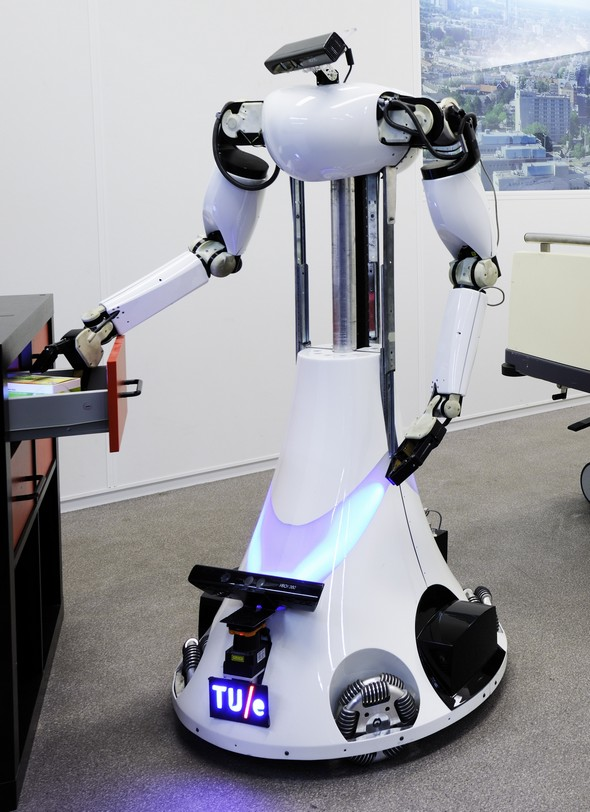
\includegraphics[width=0.3\textwidth]{amigo}
	\caption{The Amigo Robot}
	\label{fig:amigo}
\end{wrapfigure}

AMIGO (Autonomous Mate for Intelligent Operations, see Fig.~\ref{fig:amigo}) has competed in RoboCup@Home since 2011. Its design is based on a Middle Size League soccer robot, equipped with two Philips\texttrademark \hspace{0em} Experimental Robotic Arms mounted on an extensible upper body. Based on our experiences with AMIGO, SERGIO (Second Edition Robot for Generic Indoor Operations, has been developed. The main differences with AMIGO are the use of Mecanum wheels which are compliantly suspended, the torso with two degrees of freedom and the modular setup. The core specifications of AMIGO are shown in Table~\ref{tab:hardwarespec}. More details about the robots are on the Robotic Open Platform\footnote{\texttt{http://www.roboticopenplatform.org/}}, where all CAD drawings, electrical schematics and CAD files are published. SERGIO will not enter the competition this year. \\

\begin{table}[H]
    \begin{center}
    \caption{Core specifications of AMIGO}
    \label{tab:hardwarespec}
    \renewcommand{\arraystretch}{1.0}
    \setlength{\tabcolsep}{5pt}
        \begin{tabular}{p{0.2\textwidth} p{0.4\textwidth}}
            \toprule
            & AMIGO \\
            \midrule
            Name & Autonomous Mate for IntelliGent Operations \\
            Base & Fully holonomic omni-wheel platform  \\
            Torso & 1 vertical DoF using a ball screw \\
            Manipulators & 2 7-DoF Philips\texttrademark \hspace{0em} Experimental Robotic Arms \\
            Neck & Pan-tilt unit using two Dynamixel RX-64 servo actuators \\
            Head & Microsoft Kinect\texttrademark \hspace{0em} for XBox 360\texttrademark \\
            External devices & Wireless emergency button \\
            Dimensions & Diameter: $0.75\ \mathrm{m}$, height: $\pm1.5\ \mathrm{m}$ \\
            Weight & $\pm84\ \mathrm{kg}$ \\
            Additional sensors & Hokuyo UTM-30LX laser range finder on base and torso\\
            Microphone & R{\O}DE Videomic and Matrix Creator\\
            Batteries & $4\times$ Makita $24\ \mathrm{V},\ 3.3\ \mathrm{Ah}$ \\
            Computers & $3\times$ AOpen Mini PC with Core-i7 processor and $8\ \mathrm{GB}$ RAM and NVidia Jetson TX2 \\
            \bottomrule
        \end{tabular}
    \end{center}
\end{table}

\newpage
\section*{Amigo's Software Description}
% Please describe in this section the software you are using to control your robot. Consider the following example:

An overview of the software used by the Tech United Eindhoven @Home robots is shown in Table~\ref{tab:softwarespec}.
All our software is developed open-source on GitHub\footnote{\url{https://github.com/tue-robotics}}.
\\\newline
Some \textit{image\_recognition} packages are released into the ROS Kinetic distribution and can be installed with use of \textit{apt}.\\


\begin{table}[H]
    \begin{center}
    \caption{Software overview of Amigo.}
    \label{tab:softwarespec}
    %\vspace{-0.1cm}
    \renewcommand{\arraystretch}{1.0}
    \setlength{\tabcolsep}{5pt}
        \begin{tabular}{p{0.3\textwidth} p{0.7\textwidth}}
            \toprule
            Operating system & Ubuntu 16.04 LTS Server\\

            Middleware & ROS Kinetic~\cite{Quigley2009}\\

            Low-level control software & Orocos Real-Time Toolkit~\cite{Bruyninckx2001}\newline
            \url{https://github.com/tue-robotics/rtt_control_components}
            \\

            Simulation & Custom kinematics + sensor simulator \newline
            \url{https://github.com/tue-robotics/fast_simulator}
            \\

            World model & \acrfull{ed}, custom \newline
            \url{https://github.com/tue-robotics/ed}\\

            Localization & Monte Carlo~\cite{Fox2003} using \gls{ed}, custom \newline \url{https://github.com/tue-robotics/ed_localization}\\

            SLAM & Gmapping package \newline \url{http://wiki.ros.org/gmapping}\\

            Navigation & CB Base navigation
            \newline
            \url{https://github.com/tue-robotics/cb_base_navigation}
            \newline
            Global: custom A* planner\newline Local: modified ROS DWA~\cite{Fox1997}\\

            Arm navigation & Custom implementation using MoveIt and Orocos KDL\newline
            \url{https://github.com/tue-robotics/tue_manipulation}
            \\

            Object recognition & Tensorflow ROS \newline
			\url{https://github.com/tue-robotics/image_recognition/tree/master/tensorflow_ros}\\

            People detection & Custom implementation using contour matching \newline
            \url{https://github.com/tue-robotics/ed_perception}
            \\
            Face detection \& recognition & Openface ROS \newline \url{https://github.com/tue-robotics/image_recognition/tree/master/openface_ros} \\

            Speech recognition & Dragonfly + Windows\texttrademark \hspace{0em} Speech Recognition \newline
            \url{https://github.com/tue-robotics/dragonfly_speech_recognition}\\
            Speech synthesis & \texttrademark \hspace{0em} Text-to-Speech\\
            Task executors & SMACH \newline
            \url{https://github.com/tue-robotics/tue_robocup}\\
            \bottomrule
        \end{tabular}
    \end{center}
\end{table}

\section*{External Devices}
% Please describe in this section the external devices used by your robot. Consider the following example:

\textit{Amigo relies on the following external hardware:}

\begin{itemize}
	\item Tyro 2-channel wireless emergency stop (\url{https://www.tyroremotes.nl})
	\item Apple iPad for the web GUI (\url{https://www.apple.com})
\end{itemize}

\section*{Cloud Services}
% Please describe in this section the Cloud Services and online software used by your robot. Consider the following example:

\textit{Amigo connects the following cloud services:}
\begin{itemize}
   \item Skybiometry face detection (\url{https://skybiometry.com/})
\end{itemize} 